\documentclass[journal,12pt,twocolumn]{IEEEtran}

\usepackage{setspace}
\usepackage{gensymb}
\usepackage{standalone}
\singlespacing


\usepackage[cmex10]{amsmath}

\usepackage{amsthm}
\usepackage{mathrsfs}
\usepackage{txfonts}
\usepackage{stfloats}
\usepackage{bm}
\usepackage{cite}
\usepackage{cases}
\usepackage{subfig}

\usepackage{longtable}
\usepackage{multirow}

\usepackage{enumitem}
\usepackage{mathtools}
\usepackage{steinmetz}
\usepackage{tikz}
\usepackage{circuitikz}
\usepackage{verbatim}
\usepackage{tfrupee}
\usepackage[breaklinks=true]{hyperref}
\usepackage{graphicx}
\usepackage{tkz-euclide}

\usetikzlibrary{calc,math}
\usepackage{listings}
    \usepackage{color}                                            %%
    \usepackage{array}                                            %%
    \usepackage{longtable}                                        %%
    \usepackage{calc}                                             %%
    \usepackage{multirow}                                         %%
    \usepackage{hhline}                                           %%
    \usepackage{ifthen}                                           %%
    \usepackage{lscape}     
\usepackage{multicol}
\usepackage{chngcntr}

\DeclareMathOperator*{\Res}{Res}

\renewcommand\thesection{\arabic{section}}
\renewcommand\thesubsection{\thesection.\arabic{subsection}}
\renewcommand\thesubsubsection{\thesubsection.\arabic{subsubsection}}

\renewcommand\thesectiondis{\arabic{section}}
\renewcommand\thesubsectiondis{\thesectiondis.\arabic{subsection}}
\renewcommand\thesubsubsectiondis{\thesubsectiondis.\arabic{subsubsection}}


\hyphenation{op-tical net-works semi-conduc-tor}
\def\inputGnumericTable{}                                 %%

\lstset{
%language=C,
frame=single, 
breaklines=true,
columns=fullflexible
}
\usepackage{pdfpages}
\usepackage{pgfplots}

\begin{document}


\newtheorem{theorem}{Theorem}[section]
\newtheorem{problem}{Problem}
\newtheorem{proposition}{Proposition}[section]
\newtheorem{lemma}{Lemma}[section]
\newtheorem{corollary}[theorem]{Corollary}
\newtheorem{example}{Example}[section]
\newtheorem{definition}[problem]{Definition}

\newcommand{\BEQA}{\begin{eqnarray}}
\newcommand{\EEQA}{\end{eqnarray}}
\newcommand{\define}{\stackrel{\triangle}{=}}
\bibliographystyle{IEEEtran}
\providecommand{\mbf}{\mathbf}
\providecommand{\pr}[1]{\ensuremath{\Pr\left(#1\right)}}
\providecommand{\qfunc}[1]{\ensuremath{Q\left(#1\right)}}
\providecommand{\sbrak}[1]{\ensuremath{{}\left[#1\right]}}
\providecommand{\lsbrak}[1]{\ensuremath{{}\left[#1\right.}}
\providecommand{\rsbrak}[1]{\ensuremath{{}\left.#1\right]}}
\providecommand{\brak}[1]{\ensuremath{\left(#1\right)}}
\providecommand{\lbrak}[1]{\ensuremath{\left(#1\right.}}
\providecommand{\rbrak}[1]{\ensuremath{\left.#1\right)}}
\providecommand{\cbrak}[1]{\ensuremath{\left\{#1\right\}}}
\providecommand{\lcbrak}[1]{\ensuremath{\left\{#1\right.}}
\providecommand{\rcbrak}[1]{\ensuremath{\left.#1\right\}}}
\theoremstyle{remark}
\newtheorem{rem}{Remark}
\newcommand{\sgn}{\mathop{\mathrm{sgn}}}
\providecommand{\abs}[1]{\left\vert#1\right\vert}
\providecommand{\res}[1]{\Res\displaylimits_{#1}} 
\providecommand{\norm}[1]{\left\lVert#1\right\rVert}
%\providecommand{\norm}[1]{\lVert#1\rVert}
\providecommand{\mtx}[1]{\mathbf{#1}}
\providecommand{\mean}[1]{E\left[ #1 \right]}
\providecommand{\fourier}{\overset{\mathcal{F}}{ \rightleftharpoons}}
%\providecommand{\hilbert}{\overset{\mathcal{H}}{ \rightleftharpoons}}
\providecommand{\system}{\overset{\mathcal{H}}{ \longleftrightarrow}}
	%\newcommand{\solution}[2]{\textbf{Solution:}{#1}}
\newcommand{\solution}{\noindent \textbf{Solution: }}
\newcommand{\cosec}{\,\text{cosec}\,}
\providecommand{\dec}[2]{\ensuremath{\overset{#1}{\underset{#2}{\gtrless}}}}
\newcommand{\myvec}[1]{\ensuremath{\begin{pmatrix}#1\end{pmatrix}}}
\newcommand{\mydet}[1]{\ensuremath{\begin{vmatrix}#1\end{vmatrix}}}
\numberwithin{equation}{subsection}
\makeatletter
\@addtoreset{figure}{problem}
\makeatother
\let\StandardTheFigure\thefigure
\let\vec\mathbf
\renewcommand{\thefigure}{\theproblem}
\def\putbox#1#2#3{\makebox[0in][l]{\makebox[#1][l]{}\raisebox{\baselineskip}[0in][0in]{\raisebox{#2}[0in][0in]{#3}}}}
     \def\rightbox#1{\makebox[0in][r]{#1}}
     \def\centbox#1{\makebox[0in]{#1}}
     \def\topbox#1{\raisebox{-\baselineskip}[0in][0in]{#1}}
     \def\midbox#1{\raisebox{-0.5\baselineskip}[0in][0in]{#1}}
\vspace{3cm}
\title{Assignment 6}
\author{AVVARU BHARAT}
\maketitle
\newpage
\bigskip
\renewcommand{\thefigure}{1}
\renewcommand{\thetable}{\theenumi}
Download latex-tikz codes from 
%
\begin{lstlisting}
https://github.com/Bharat437/Matrix_Theory/tree/master/Assignment6
\end{lstlisting}
\section{\textbf{Question}}
(Ramsey 3.4.4)Q. What does the equation
\begin{align}
    \vec{x^T}\myvec{ 1 & \sqrt{3} \\ \sqrt{3} & -1 }\vec{x}=2a^2\label{eq:given}
\end{align}
become when the axes are turned through $30\degree$
\section{\textbf{Explanation}}
The general second degree equation is expressed as follows,
\begin{align}
    \vec{x^TVx}+2\vec{u^Tx}+f=0\label{eq:gen}
\end{align}
Comparing \eqref{eq:given} and \eqref{eq:gen}, we get
\begin{align}
    \vec{V}=\myvec{ 1 & \sqrt{3} \\ \sqrt{3} & -1 }\label{eq:V}\\
    \vec{u}=\myvec{0 \\ 0}\label{eq:u}\\
    f=-2a^2\label{eq:f}
\end{align}
Now we find
\begin{align}
    \mydet{\vec{V}}=\mydet{1 & \sqrt{3} \\ \sqrt{3} & -1}\\
    \implies\mydet{\vec{V}}=-4\\
    \implies\mydet{\vec{V}}<0
\end{align}

Therefore the given equation \eqref{eq:given} represents  hyperbola.

Now from affine transformations,
\begin{align}
    \vec{x}=\vec{Py}+\vec{c}
\end{align}

We have to rotate the axes by $\theta=30\degree$, Then using rotation matrix.
\begin{align}
    \vec{P}=\myvec{\cos\theta & -\sin\theta \\ \sin\theta & \cos\theta}
\end{align}
\begin{align}
    \implies\vec{P}=\myvec{\cos30\degree & -\sin30\degree \\ \sin30\degree & \cos30\degree}\\
    \implies\vec{P}=\myvec{\frac{\sqrt{3}}{2} & -\frac{1}{2} \\ \frac{1}{2} & \frac{\sqrt{3}}{2}}\label{eq:P}
\end{align}

From eigenvalue decomposition,
\begin{align}
    \vec{P^TVP}=\vec{D}\label{eq:eigval}
\end{align}
\begin{align}
    \implies\vec{D}=\myvec{\frac{\sqrt{3}}{2} & \frac{1}{2} \\ -\frac{1}{2} & \frac{\sqrt{3}}{2}}\myvec{1 & \sqrt{3} \\ \sqrt{3} & -1}\myvec{\frac{\sqrt{3}}{2} & -\frac{1}{2} \\ \frac{1}{2} & \frac{\sqrt{3}}{2}}\\
    \implies\vec{D}=\myvec{2 & 0 \\ 0 & -2}=\myvec{\lambda_1 & 0 \\ 0 & \lambda_2}\label{eq:D}
\end{align}
\begin{align}
    \vec{P}=\myvec{\vec{p_1} & \vec{p_2}}\\
    \vec{P}^T=\vec{P}^{-1}
\end{align}

The equation \eqref{eq:gen} becomes as below due to affine transformation
\begin{align}
    \vec{y}^T\vec{Dy}=\vec{u}^T\vec{V}^{-1}\vec{u}-f\label{eq:trans}
\end{align}
with 
\begin{align}
    \vec{c}=-\vec{V}^{-1}\vec{u}\label{eq:ctrans}
\end{align}
\renewcommand{\thefigure}{1}
\begin{figure}[ht!]
    \centering
    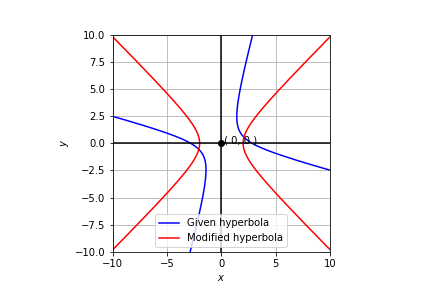
\includegraphics[width=\columnwidth]{Figure}
    \caption{Hyperbola when rotated by $30\degree$}
    \label{fig:figure1}
\end{figure}\\
Substitute \eqref{eq:V},\eqref{eq:u},\eqref{eq:f},\eqref{eq:D} in \eqref{eq:trans} and \eqref{eq:ctrans}, we get
\begin{align}
    \vec{y}^T\myvec{2 & 0 \\ 0 & -2}\vec{y}=2a^2\label{eq:T}
\end{align}
with centre,
\begin{align}
    \vec{c}=\myvec{0 \\ 0}
\end{align}

Therefore the given equation \eqref{eq:given} becomes \eqref{eq:T} when the axes are turned through $30\degree$.

The plot is shown in Fig ~\ref{fig:figure1}
\end{document}
